\documentclass{article}

% if you need to pass options to natbib, use, e.g.:
%     \PassOptionsToPackage{numbers, compress}{natbib}
% before loading neurips_2018

% ready for submission
% \usepackage{nips_2018}

% to compile a preprint version, e.g., for submission to arXiv, add add the
% [preprint] option:
%     \usepackage[preprint]{neurips_2018}

% to compile a camera-ready version, add the [final] option, e.g.:
    \usepackage[final]{nips_2018}
% to avoid loading the natbib package, add option nonatbib:
     %\usepackage[nonatbib]{neurips_2018}

\usepackage[italian]{babel}

\usepackage[utf8]{inputenc} % allow utf-8 input
\usepackage[T1]{fontenc}    % use 8-bit T1 fonts
\usepackage{hyperref}       % hyperlinks
\usepackage{url}            % simple URL typesetting
\usepackage{booktabs}       % professional-quality tables
\usepackage{amsfonts}       % blackboard math symbols
\usepackage{nicefrac}       % compact symbols for 1/2, etc.
\usepackage{microtype}      % microtypography
\usepackage{graphicx}
\usepackage{subcaption}
\usepackage{booktabs}
\title{Classificazione di Strumenti Musicali con Reti Convoluzionali}


% The \author macro works with any number of authors. There are two commands
% used to separate the names and addresses of multiple authors: \And and \AND.
%
% Using \And between authors leaves it to LaTeX to determine where to break the
% lines. Using \AND forces a line break at that point. So, if LaTeX puts 3 of 4
% authors names on the first line, and the last on the second line, try using
% \AND instead of \And before the third author name.

\author{%
  Giuseppe De Palma \\
  Matricola: 854668 \\
  Corso di Laurea Magistrale in Informatica \\
  Machine Learning A.A. 2018/2019 \\
  \texttt{giuseppe.depalma@studio.unibo.it}
  % examples of more authors
  \And
  Alessandro Liberato \\
  Matricola: 842906 \\
  Corso di Laurea Magistrale in Informatica \\
  Machine Learning A.A. 2018/2019 \\
  \texttt{alessandro.liberato@studio.unibo.it} 
  % \AND
  % Coauthor \\
  % Affiliation \\
  % Address \\
  % \texttt{email} \\
  % \And
  % Coauthor \\
  % Affiliation \\
  % Address \\
  % \texttt{email} \\
  % \And
  % Coauthor \\
  % Affiliation \\
  % Address \\
  % \texttt{email} \\
}

\begin{document}
% \nipsfinalcopy is no longer used

\maketitle
\section{Introduzione}
Lo scopo di questo progetto è stato quello di riprendere un lavoro di tesi passato e, sugli stessi task e dati,
applicare delle tecniche di uso comune che in precedenza (nel periodo della tesi) erano appena emergenti e non consolidate.
Tali tecniche riguardano la \textit{image classification} utilizzando reti convoluzionali, nella fattispecie applicando la metodologia del transfer learning.
Il livello raggiunto oggigiorno dell'accoppiata reti convoluzionali e transfer learning è davvero molto alto.
Quindi, il task del progetto è stato quello di addestrare reti neurali convoluzionali al riconoscimento di strumenti
musicali, a partire da dataset composti da singole note. I risultati raggiunti al termine del progetto sono da considerarsi
più che soddisfacenti.

\section{Dataset}

Inizialmente il lavoro di tesi su cui si basa il progetto attingeva i dati da diversi dataset composti da file audio di note di strumenti musicali 
di musica classica, il terzo dei quali, allo stato attuale,
risulta inaccessibile (Vienna Symphonic Library). Le tecniche utilizzate nel lavoro precedente vedevano i risultati migliori proprio
con l'utilizzo del suddetto dataset, tuttavia nel nostro progetto tale mancanza è risultata ininfluente (proprio grazie ai nuovi metodi).

\subsection{Fonti dei dati}
I dati per questo progetto provengono da:
\begin{itemize}
    \item The University of Iowa
    \item Sonatina Symphonic Orchestra
\end{itemize}
Ai fini del progetto, senza perdita di generalità, abbiamo ridotto lo scope degli strumenti considerati a 4 (fagotto, flauto, pianoforte, trombone), 
per motivi di risorse computazionali limitate e scarsità di file audio per specifici strumenti (strumenti molto particolari).

\subsection{Pre-processing dei dati}
Una delle novità è stata quella di utilizzare tecniche di riconoscimento basate su immagini invece che sui suoni.
Un modo per visualizzare un segnale sonoro è quello di rappresentarlo graficamente per mezzo di 3 parametri: intensità, frequenza e tempo (ovvero per mezzo
di spettrogrammi).
\clearpage
Di seguito questi sono 4 esempi rappresentativi:
\begin{figure}[h]
    \centering
    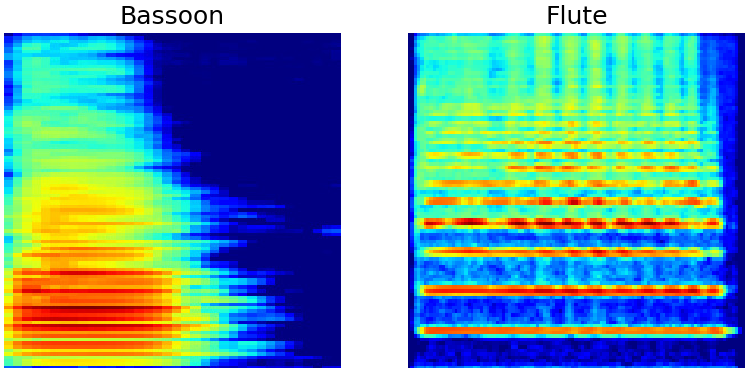
\includegraphics[scale=0.5]{immagini/classes_samples_1.png}
    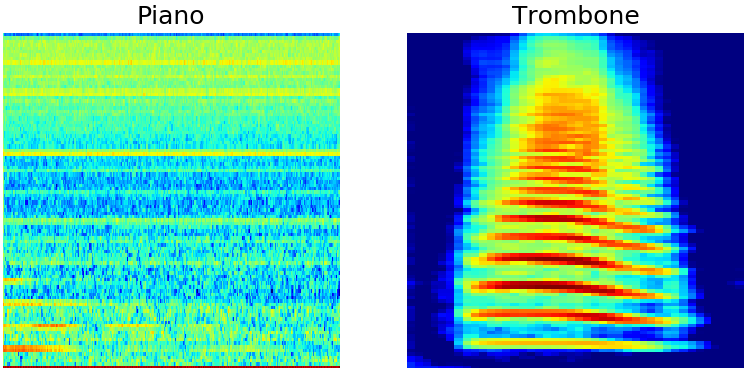
\includegraphics[scale=0.5]{immagini/classes_samples_2.png}
    \caption{\textit{Spettrogrammi di 4 clip audio di 10 secondi, una per ogni strumento da classificare.}}
\end{figure}

Le fasi di manipolazione dei file audio nativi dei dataset sono le seguenti:
\begin{itemize}
    \item Conversione da formati aif e aiff in formato wav:\\
    Tutti i file dei dataset raccolti sono alcuni in formati aif ed altri in aiff, per questo motivo si è voluto convertire 
    tutti i file in un unico formato più comune, optando per wav. Questo è stato svolto utilizzando il tool \textit{ffmpeg} da terminale bash. 
    Il formato wav è stato scelto per via della compatibilità con il codice scritto in precedenza per creare spettrogrammi, tramite la libreria \textit{librosa}.
    \item Splitting dei file wav in clip da 10 secondi o meno ognuna:\\
    Questa fase è stata necessaria per via della variabilità delle durate dei file audio (da meno di 10 secondi ad anche più di 1 minuto).
    Le registrazioni degli strumenti coprono le singole note, ciascuna delle quali anche in più di una tecnica (es. pizzicato).
    Per questo motivo è stato deciso di uniformare i file per la creazione degli spettrogrammi in clip audio da massimo 10 secondi, durata ritenuta sufficiente 
    avere abbastanza informazioni per la creazione di spettrogrammi utili. La procedura di ``clipping'' è stata eseguita con 
    \textit{ffmpeg} da terminale bash.  
    \item Conversione di ciascuna clip in spettrogramma in formato png:\\
    La creazione di spettrogrammi è stata eseguita tramite i tool Librosa e Matplotlib. Il primo è uno strumento di music information retrieval che a partire
    da un file audio estrae i dati necessari da passare a matplotlib per poter renderizzare uno spettogramma.
    \item Conversione di ciascuno spettrogramma png in formato jpg:\\
    Abbiamo usato il tool \textit{mogrify} da terminale bash per convertire il formato delle immagini. 
    Ciò è stato necessario in quanto bisogna avere immagini
    senza la quarta componente della trasparenza, ma solo RGB, per questioni di compatibilità con il layer di input della rete. 
    \item Ridenominazione di ciascuno spettrogramma:\\
    Infine tutti gli spettrogrammi sono stati accorpati in un'unica directory per il training, e ridenominati per estrarre la classe di appartenenza 
    e assegnare un ID univoco.
\end{itemize}

Tali passaggi sono stati necessari per motivi di compatibilità con le tecniche utilizzate (creazione spettrogrammi e riconoscimento immagini).

\section{Metodo Utilizzato}
Dato che ciascuno strumento musicale conserva delle caratteristiche pressochè uniche anche quando il suo suono viene tradotto in spettrogramma,
è sensato lavorare con delle reti adatte alla classificazione di immagini. Tra le migliori ci sono le reti convoluzionali.

\subsection{Reti Convoluzionali}
Le reti convoluzionali consistono di blocchi che alternano le seguenti operazioni:
convoluzione e pooling. L'operazione di convoluzione avviene facendo scorrere un filtro lineare sulle immagini di input di dimensione fissata,
eseguendo una moltiplicazione element-wise tra il filtro e l'immagine, dopo la quale i risultati intermedi vengono sommati per ottenere un unico valore
che rappresenta una feature dell'immagine. Queste features saranno imparate durante il training dalla rete per mezzo del classico algoritmo di backpropagation.
L'operazione di pooling, invece, consiste nella riduzione della dimensione della features map ottenuta dai passi di convoluzione. 
Tipicamente, ciò che si fa è max pooling con finestra 2x2.  

La convoluzione è di per se lineare e quindi è necessario, per rendere la rete più potente, introdurre una qualche componente non lineare.
A tale scopo nella rete si utilizza la funzione di attivazione ReLU. 

\subsection{VGG-16}
Il primo modello che abbiamo utilizzato è VGG-16, che è una delle più performanti reti convoluzionali allo stato attuale.
Tale rete è composta da 5 blocchi convoluzionali (la base convoluzionale) seguita da un insieme di layer con un alta densità di connessioni,
il cui output sono le probabilità che una immagine appartiene a ciascuna classe.
Nello specifico, la parte terminale della rete (quella dopo i blocchi convoluzionali) è stata modificata nel modo illustrato in figura 2, 
ovvero adattata per il riconoscimento delle note musicali con delle accortezze atte ad evitare over-fitting. Questa particolare topologia della rete
è stata ottenuta e riadattata dal paper da cui questo progetto ha preso ispirazione e spunto \cite{paper}. Tra le particolarità
è presente un layer di dropout nella parte finale della rete con lo scopo di evitare overfitting. Dato che le prestazioni della rete non si sono degradate
con questa topologia, abbiamo ritenuto opportuno lasciare la rete invariata.

\begin{figure}[h]
    \centering
    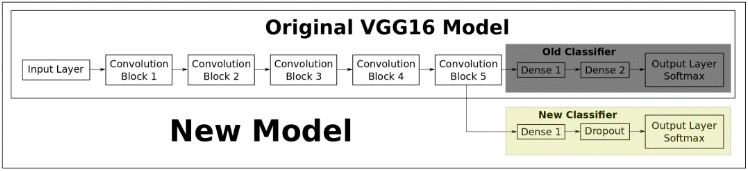
\includegraphics[width=\linewidth]{immagini/vgg16.png}
    \caption{Architettura della rete VGG-16 modificata.}
    \label{nn:vgg}
\end{figure}

\subsection{InceptionV3}
Come ulteriore task, si è affrontato il solito problema della classificazione degli strumenti musicali utilizzando
un'altra rete convoluzionale: InceptionV3, la cui architettura è quella in figura 3.
La differenza principale oltre l'architettura è la minore richiesta di potere computazionale per svolgere la fase di training, con una degradazione trascurabile delle prestazioni.
\clearpage
\begin{figure}[h]
    \centering
    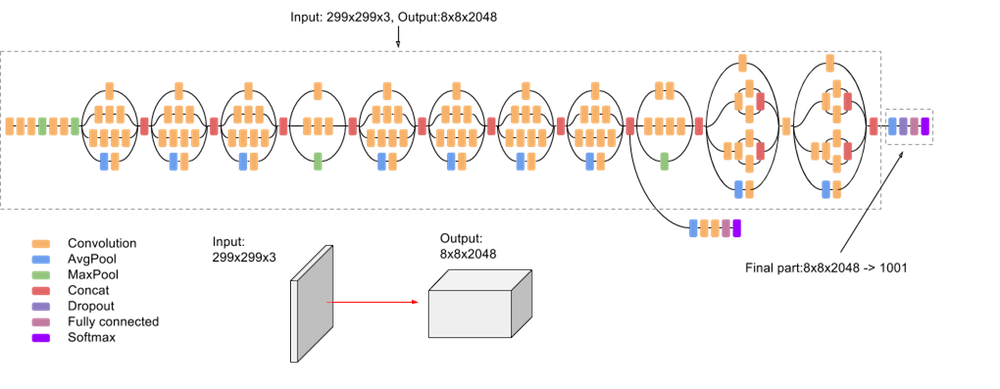
\includegraphics[width=\linewidth]{immagini/incv3.png}
    \caption{Architettura della rete InceptionV3.}
    \label{nn:inc}
\end{figure}
\subsection{Training}
La metodologia di training utilizzata è stata quella del transfer learning, che consiste nel tenere fissati
i pesi della base convoluzionale ottenuti da una rete pre-addestrata su ImageNet. A seguito dell'acquisizione
di tali i pesi, si è allenata solamente l'ultima parte della rete per la classificazione dei 4 strumenti scelti, per la durata di 10 epoch.
Questo è stato fatto sia in cloud con servizi forniti da AWS (Amazon Web Services), sia su una macchina in locale 
con 16GB di RAM e CPU Intel Core i7 7500U. Il training completo per VGG-16 per classificare i 4 struemnti ha richiesto circa 1 ora per ogni epoch, raggiungendo poco più di 10 ore
per completare la fase di training. InceptionV3 invece è stato in totale più veloce, quasi dimezzando il tempo arrivando a 6 ore in totale per ogni training totale effettuato.

\section{Risultati}
I risultati ottenuti sono rappresentati nelle seguenti confusion matrix:

\begin{figure}[h]
    \centering
    \begin{subfigure}{.5\textwidth}
      \centering
      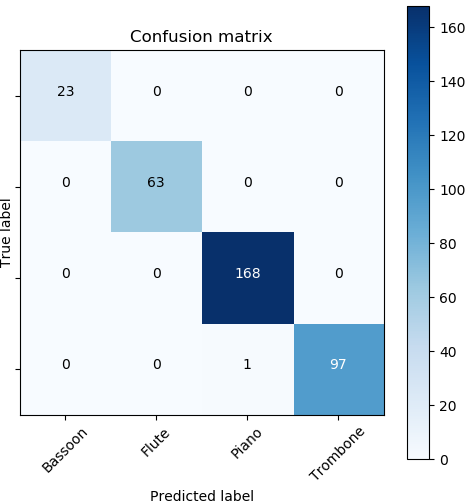
\includegraphics[scale=0.5]{immagini/vgg16_confusion_matrix.png}
      \caption{VGG-16}
    \end{subfigure}%
    \begin{subfigure}{.5\textwidth}
      \centering
      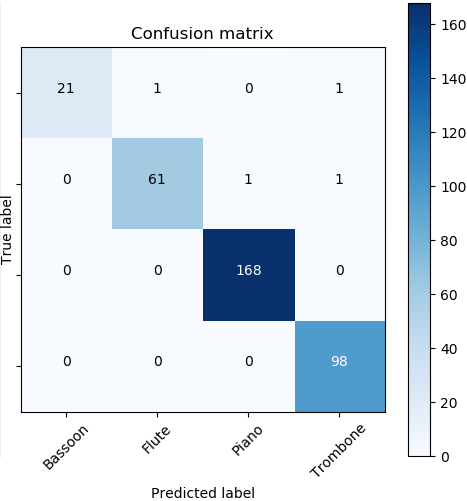
\includegraphics[scale=0.5]{immagini/incv3_confusion_matrix.png}
      \caption{InceptionV3}
    \end{subfigure}
    \caption{Le confusion matrix delle due reti.}
    \label{fig:matrices}
\end{figure}
\clearpage
Dalla figura 4 emerge che l'esito di entrambi i training è da considerarsi molto positivi. I test sono stati eseguiti sul 30\% del totale dei dati,
raggiungendo le seguenti accuratezze:
\begin{itemize}
    \item VGG-16: 98,44\%
    \item InceptionV3: 96,09\%
\end{itemize}
In aggiunta a tali valutazioni, abbiamo sviluppato uno script che, presi i dati da un dataset sconosciuto al modello (Philarmonia Orchestra) 
effettua la classificazione di ciascuno strumento su un numero fissato di campioni presi casualmente. Anche in questo caso,
empiricamente, abbiamo riscontrato delle prestazioni nel complesso soddisfacenti. 

\subsection{Confronto Lavoro Precedente}
La migliore tecnica usata nel lavoro di tesi per classificare strumenti non a percussione, è quella della \texttt{tree-entropy}. Nella tabella \ref{tab:acc}
sono riportate le accuracy relative agli strumenti che abbiamo classificato nel nostro progetto.
\renewcommand{\arraystretch}{1.2}
\begin{table}[h]
    \centering
    \caption{Accuratezza Tree-Entropy.}
    \vspace*{3mm}
    \begin{tabular}{ c c } % suppress vertical whitespace at start and end
        \toprule
        Strumento & Accuracy \\
        \hline
        Trombone & 42.37\% \\
        Piano & 93.86\% \\
        Flauto & 61.59\% \\
        Fagotto & 46.63\% \\ 
        %\midrule[\heavyrulewidth] % use "thick" \midrule instead of \bottomrule
        \bottomrule
    \end{tabular}
    \label{tab:acc}
\end{table} \\
La nostra miglior tecnica (VGG-16) raggiunge un accuratezza totale del 98,44\% e dalla confusion matrix si nota che per ogni strumento non ci sono quasi mai errori.
Quindi le reti convoluzionali testate, con la tecnica usata degli spettrogrammi, riescono a superare, anche di molto per alcuni strumenti, le performance del modello utilizzato nella tesi.

\section{Conclusioni}
L'esito del progetto ha dimostrato che le nuove tecniche di riconoscimento immagini funzionano bene anche per manipolare 
segnali sonori codificati per mezzo di spettrogrammi, rispetto alle metodologie classiche
utilizzate al lavoro di tesi preso come metro di paragone. Questo progetto mostra una nuova strada per il riconoscimento
di strumenti, anche se con un insieme ridotto, facendo notare che tecniche ben consolidate per altri ambiti possono essere 
riadattate, ottenendo ottimi risultati.

\subsection{Possibili Miglioramenti}
I possibli miglioramenti che si possono apportare sono i seguenti:
\begin{itemize}
    \item Eseguire un taglio più accurato dei file audio rispetto al loro contenuto.
    \item Provare diverse risoluzioni degli spettrogrammi.
    \item Aumentare i dati relativi agli strumenti particolari che presentano una scarsità sostanziale dei relativi file audio.
    \item Addestrare la rete non più su singole note ma su intere composizioni (sempre di una tipologia fissata di strumenti).
\end{itemize}
La strada intrapresa in questo progetto sembra ragionevolmente promettente.   
    
\bibliographystyle{plain}
\bibliography{biblio}
        
\end{document}